%
% nichtungerade.tex
%
% (c) 2026 Damien Flury, OST Ostschweizer Fachhochschule
%
\begin{figure}
\centering
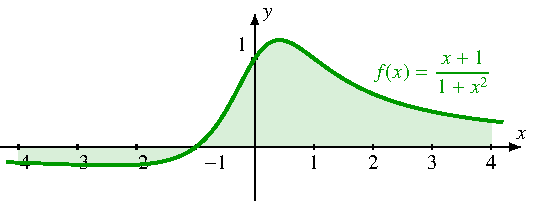
\includegraphics{papers/hauptwert/images/nichtungerade.pdf}
\caption{Graph der Funktion $f(x)=(x+1)/(1+x^2)$.
Der Integrand ist weder gerade noch ungerade;
bei symmetrischer Integration hebt sich nur sein ungerader Anteil weg.
\label{hauptwert:figure:nichtungerade}}
\end{figure}
